\section{Multipelvärdering}
\label{sec:multiplar}

En multipelvärdering \eng{comparable company analysis, trading comps} frågar inte vad bolaget
borde vara värt utan vad marknaden betalar för liknande bolag just nu. Man tar ett nyckeltal
för jämförelsebolagen \eng{peers}, till exempel rörelsevärde delat med EBITDA, och multiplicerar
med målbolagets EBITDA. Metoden är snabb, lätt att förklara och förankrad i verkliga priser.
Svagheten är densamma: om hela sektorn är felprissatt blir svaret också fel.

\subsection{Varför multiplar fungerar: en multipel är en hoptryckt DCF}

Ta Gordons formel~\eqref{eq:gordon} för ett bolag i jämvikt, $\EV = \FCFF_1/(r-g)$, och skriv
kassaflödet som en andel $\kappa$ av EBITDA, $\FCFF_1 = \kappa \cdot \EBITDA_1$. Talet $\kappa$
är kassakonverteringen \eng{cash conversion}: hur mycket av EBITDA som blir kvar efter skatt,
investeringar och rörelsekapital. Då är
\begin{equation}
  \frac{\EV}{\EBITDA_1} = \frac{\kappa}{r-g} .
  \label{eq:multipel-dcf}
\end{equation}
Multipeln är alltså inget nytt mått utan en DCF med tre antaganden hoptryckta till ett tal:
kassakonvertering, risk och tillväxt. Två bolag förtjänar samma multipel bara om de är lika i
alla tre. För Atlas Copco ger motorns slutår $\kappa = 0,62$ och $r - g = 5,65$
procentenheter, alltså 11 gånger nästa års EBITDA. Det är samma tal som den implicita
multipeln 11,7 i avsnitt~\ref{sec:gordon}, sånär som på halvårsfaktorn och ett års tillväxt.

Samma härledning för aktiekursen: utdelningen är vinsten gånger utdelningsandelen, och ett
bolag som återinvesterar andelen $g/\mathrm{ROE}$ av vinsten växer med $g$. Alltså
\begin{equation}
  \frac{P}{E_1} = \frac{1 - g/\mathrm{ROE}}{r_e - g} ,
  \label{eq:pe}
\end{equation}
där $P$ är aktiekursen, $E_1$ nästa års vinst per aktie (inte eget kapital, som $E$ betyder i
övrigt) och $\mathrm{ROE}$ avkastningen på eget kapital \eng{return on equity}. Med
$\mathrm{ROE} = 20$\pct, $g = 2$\pct{} och $r_e = 7,84$\pct{} blir P/E
$0,9 / 0,0584 = 15,4$. Jämförelsebolagen i caset handlas till 32,9 gånger vinsten. Marknaden
räknar alltså med högre tillväxt, lägre avkastningskrav eller båda.

\begin{intervjutips}
Frågan ”why would two similar companies trade at different multiples?” besvaras
med~\eqref{eq:multipel-dcf}: olika tillväxt, olika risk eller olika marginal och
kapitalbehov. Säg de tre orden \en{growth}, \en{risk} och \en{returns on capital}.
\end{intervjutips}

\subsection{Vilken multipel till vad}

Grundregeln är att täljare och nämnare ska tillhöra samma finansiärer. Rörelsevärde hör ihop
med mått före räntor (omsättning, EBITDA, EBIT). Börsvärde hör ihop med mått efter räntor
(nettoresultat, eget kapital).

\begin{table}[ht]
\centering\small
\caption{De vanligaste multiplarna. Motorn räknar de tre första.}
\label{tab:multiplar}
\begin{tabularx}{\linewidth}{@{}l>{\raggedright\arraybackslash}X>{\raggedright\arraybackslash}X@{}}
\toprule
Multipel & Använd när & Svaghet \\
\midrule
EV/EBITDA & Standardvalet för mogna rörelsedrivande bolag. Opåverkad av skuldsättning och
  avskrivningsprinciper & Bortser från hur mycket som måste investeras. Meningslös för banker \\
EV/Sales & Bolaget går med förlust eller har tillfälligt pressad marginal & Bortser helt från
  lönsamheten \\
P/E & Banker och andra finansiella bolag. Vanligast bland investerare & Påverkas av
  skuldsättning, skatt och engångsposter \\
EV/EBIT & Bolagen har olika kapitalintensitet & Påverkas av avskrivningsprinciper \\
P/B (kurs mot eget kapital) & Banker och fastighetsbolag & Säger lite om bolag med få bokförda
  tillgångar. Finns inte i motorn \\
\bottomrule
\end{tabularx}
\end{table}

\begin{vanligtfel}
Att blanda nivåerna, till exempel EV delat med nettoresultat eller börsvärde delat med EBITDA.
Lika vanligt: att jämföra multiplar som bygger på olika perioder. Motorn använder senaste
räkenskapsår för alla bolag. På en bank används oftare rullande tolv månader \eng{last twelve
months, LTM} eller nästa års prognos \eng{forward multiple}.
\end{vanligtfel}

\subsection{Klustringens matematik}

På en bank väljs jämförelsebolagen för hand av någon som kan branschen. Motorn måste klara 687
bolag utan hjälp och använder därför klustring. Tre begrepp behövs.

\paragraph{Standardisering.} Bolagen beskrivs med sex variabler: logaritmen av börsvärdet,
omsättningstillväxt, EBITDA-marginal, avkastning på eget kapital, beta och skuldsättning
($D/(D+E)$). De har helt olika skalor, och ett avstånd i rådata hade dominerats av den
variabel som råkar ha störst tal. Varje variabel $j$ räknas därför om till z-värden:
\begin{equation}
  z_{ij} = \frac{x_{ij} - \bar x_j}{s_j},
  \label{eq:z}
\end{equation}
där $\bar x_j$ och $s_j$ är medelvärde och standardavvikelse bland kandidaterna. Före
standardiseringen kapar motorn extremvärden vid 5:e och 95:e percentilen (winsorisering) och
ersätter saknade värden med medianen.

\paragraph{K-means.} Algoritmen delar punkterna $z_1, \dots, z_n$ i $k$ grupper
$C_1, \dots, C_k$ så att summan av kvadrerade avstånd till gruppens medelpunkt $\mu_j$ blir så
liten som möjligt:
\begin{equation}
  J(C_1, \dots, C_k) = \sum_{j=1}^{k} \sum_{i \in C_j} \lVert z_i - \mu_j \rVert^2,
  \qquad \mu_j = \frac{1}{|C_j|} \sum_{i \in C_j} z_i .
  \label{eq:kmeans}
\end{equation}
Att hitta det globala minimumet är NP-svårt. Lloyds algoritm hittar ett lokalt minimum genom
att växla mellan två steg:

\begin{enumerate}
  \item \textbf{Tilldela.} Varje punkt går till närmaste medelpunkt.
  \item \textbf{Uppdatera.} Varje medelpunkt flyttas till medelvärdet av sina punkter.
\end{enumerate}

Inget av stegen kan öka $J$: det första minskar varje punkts term för sig, det andra använder
att medelvärdet är den punkt som minimerar summan av kvadrerade avstånd. Eftersom $J$ är
avtagande och antalet uppdelningar är ändligt stannar algoritmen efter ändligt många steg. Men
resultatet beror på startpunkterna, så motorn kör tio starter med fast slumpfrö
(\kod{n_init=10}, \kod{random_state=42}) och behåller den bästa.

\paragraph{Silhuettvärdet} avgör hur många kluster som passar. För punkt $i$ är $a(i)$
medelavståndet till de andra punkterna i samma kluster och $b(i)$ medelavståndet till punkterna
i närmaste \emph{andra} kluster:
\begin{equation}
  s(i) = \frac{b(i) - a(i)}{\max\{a(i),\, b(i)\}} \in [-1, 1] .
  \label{eq:silhuett}
\end{equation}
Nära 1 betyder att punkten ligger tätt bland de sina och långt från andra. Nära 0 betyder att
den ligger på gränsen. Motorn prövar $k = 2, \dots, 8$ och väljer det $k$ som ger högst
medelvärde av $s(i)$.

\subsection{Hur motorn faktiskt väljer jämförelsebolag}
\label{sec:peers-arligt}

Projektet beskrivs som ”comps med k-means”. Det är sant, men klustringen gör mindre av jobbet
än namnet antyder. Så här går det till för Atlas Copco:

\begin{enumerate}
  \item \textbf{Kandidater.} Bara bolag i samma sektor enligt Yahoo (Industrials) kommer i
    fråga: 148 stycken. Utan den spärren hade klustringen kunnat para ihop en bank med ett
    bioteknikbolag av samma storlek.
  \item \textbf{Klustring.} Silhuettvärdet är högst för $k = 2$ (figur~\ref{fig:silhuett}).
    Av de 148 kandidaterna hamnar 119 i samma kluster som Atlas Copco. Klustringen sorterar
    alltså bort en femtedel och inte mer. I projektets körning över hela universumet väljs $k = 2$ för ungefär
    halva universumet.
  \item \textbf{Rangordning.} Det verkliga urvalet görs av en rangordning efter avstånd i
    z-rummet, med ett straff för annan bransch:
    $\lVert z_i - z_{\text{mål}} \rVert + 0,5 \cdot p_i$, där $p_i = 0$ för samma bransch,
    $0,5$ för samma branschfamilj, $1$ för annan bransch i sektorn och $2$ för annan sektor.
    De tolv närmaste behålls.
  \item \textbf{Rensning.} Multiplar utanför ett Tukey-staket ($1,5$ kvartilavstånd på
    logaritmen av multipeln) tas bort. Här faller ett bolag bort, Electrolux Professional, och
    elva blir kvar.
  \item \textbf{Värde.} Gruppens 25:e percentil, median och 75:e percentil multipliceras med
    målbolagets eget mått och förs genom bryggan~\eqref{eq:brygga}.
\end{enumerate}

\begin{figure}[ht]
\centering
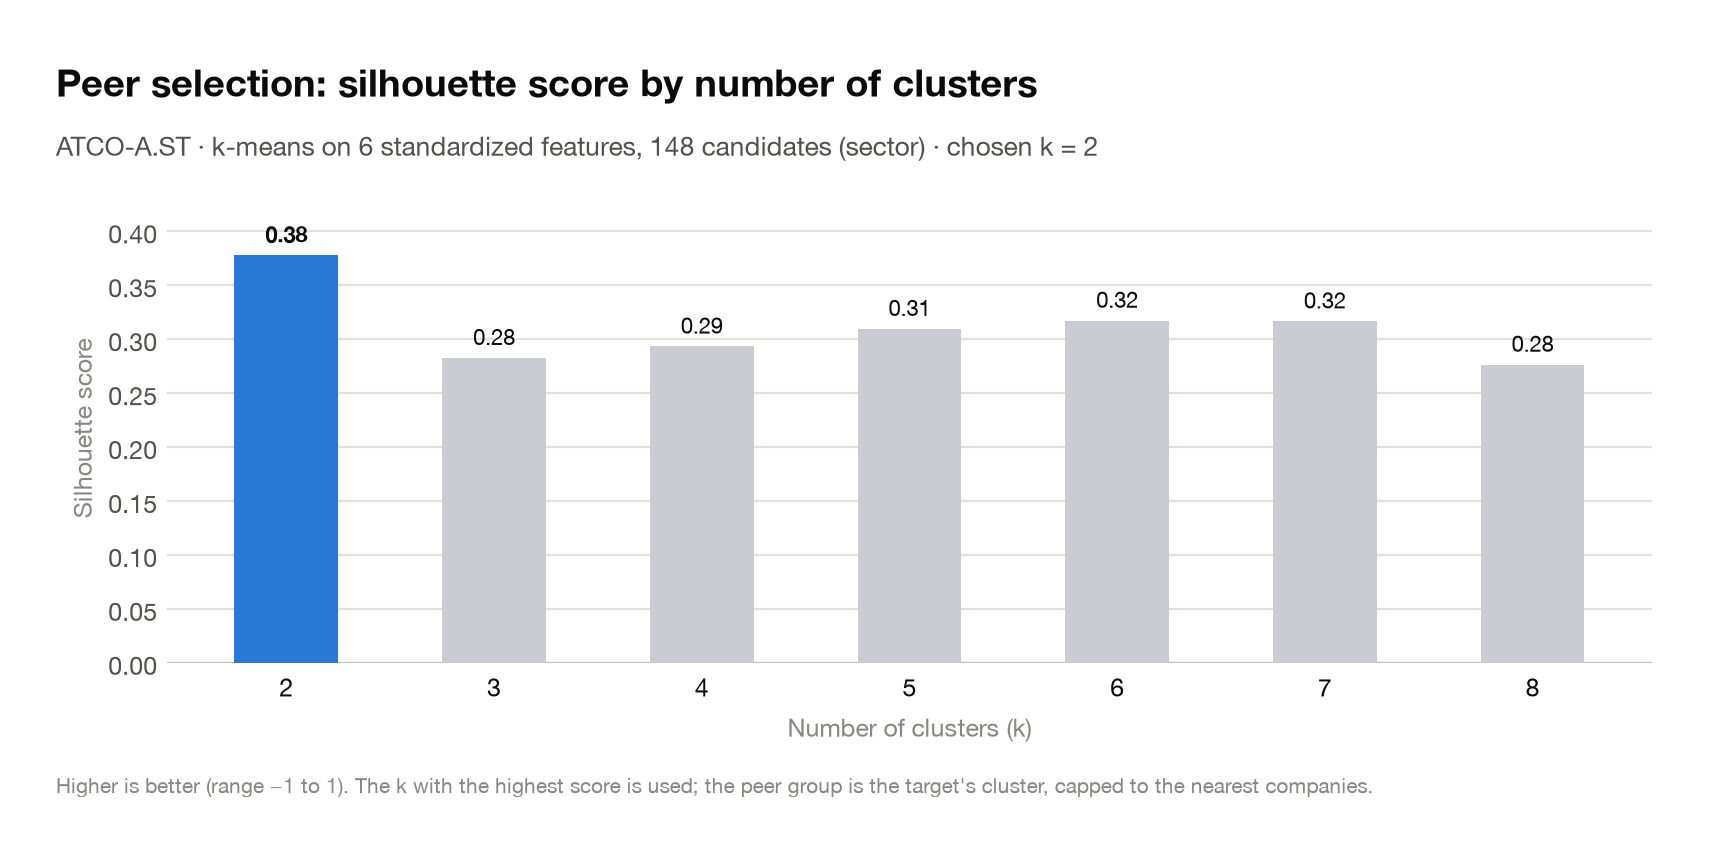
\includegraphics[width=0.72\linewidth]{comps_silhouette.png}
\caption{Silhuettvärde per antal kluster för Atlas Copcos sektor. $k = 2$ vinner, men inget
värde är högt: det finns ingen tydlig klusterstruktur i data.}
\label{fig:silhuett}
\end{figure}

\begin{komihag}
Ärligt beskrivet väljer motorn jämförelsebolag med \emph{närmaste grannar inom sektorn, med
förtur för samma bransch}. K-means bidrar med en grov första sållning. Säg det så i en
intervju. Det är mer trovärdigt än att påstå att en klustringsalgoritm har hittat de rätta
bolagen.
\end{komihag}

Resultatet för Atlas Copco är en blandad grupp: Sandvik, Alfa Laval, Epiroc, Trelleborg,
Mycronic, Lifco, Addtech, Indutrade, Latour, Beijer Alma och Assa Abloy. Alla är mindre än
Atlas Copco, och ett av dem är ett investmentbolag. Figur~\ref{fig:comps} visar deras multiplar.
Räkningen för EV/EBITDA: medianen 19,4 gånger Atlas Copcos EBITDA 44,1~mdkr ger ett
rörelsevärde på 856,6~mdkr. Minus nettoskuld och minoritet (12,6) blir aktievärdet 844,0~mdkr,
eller 172,9\kr{} per aktie.

\begin{figure}[ht]
\centering
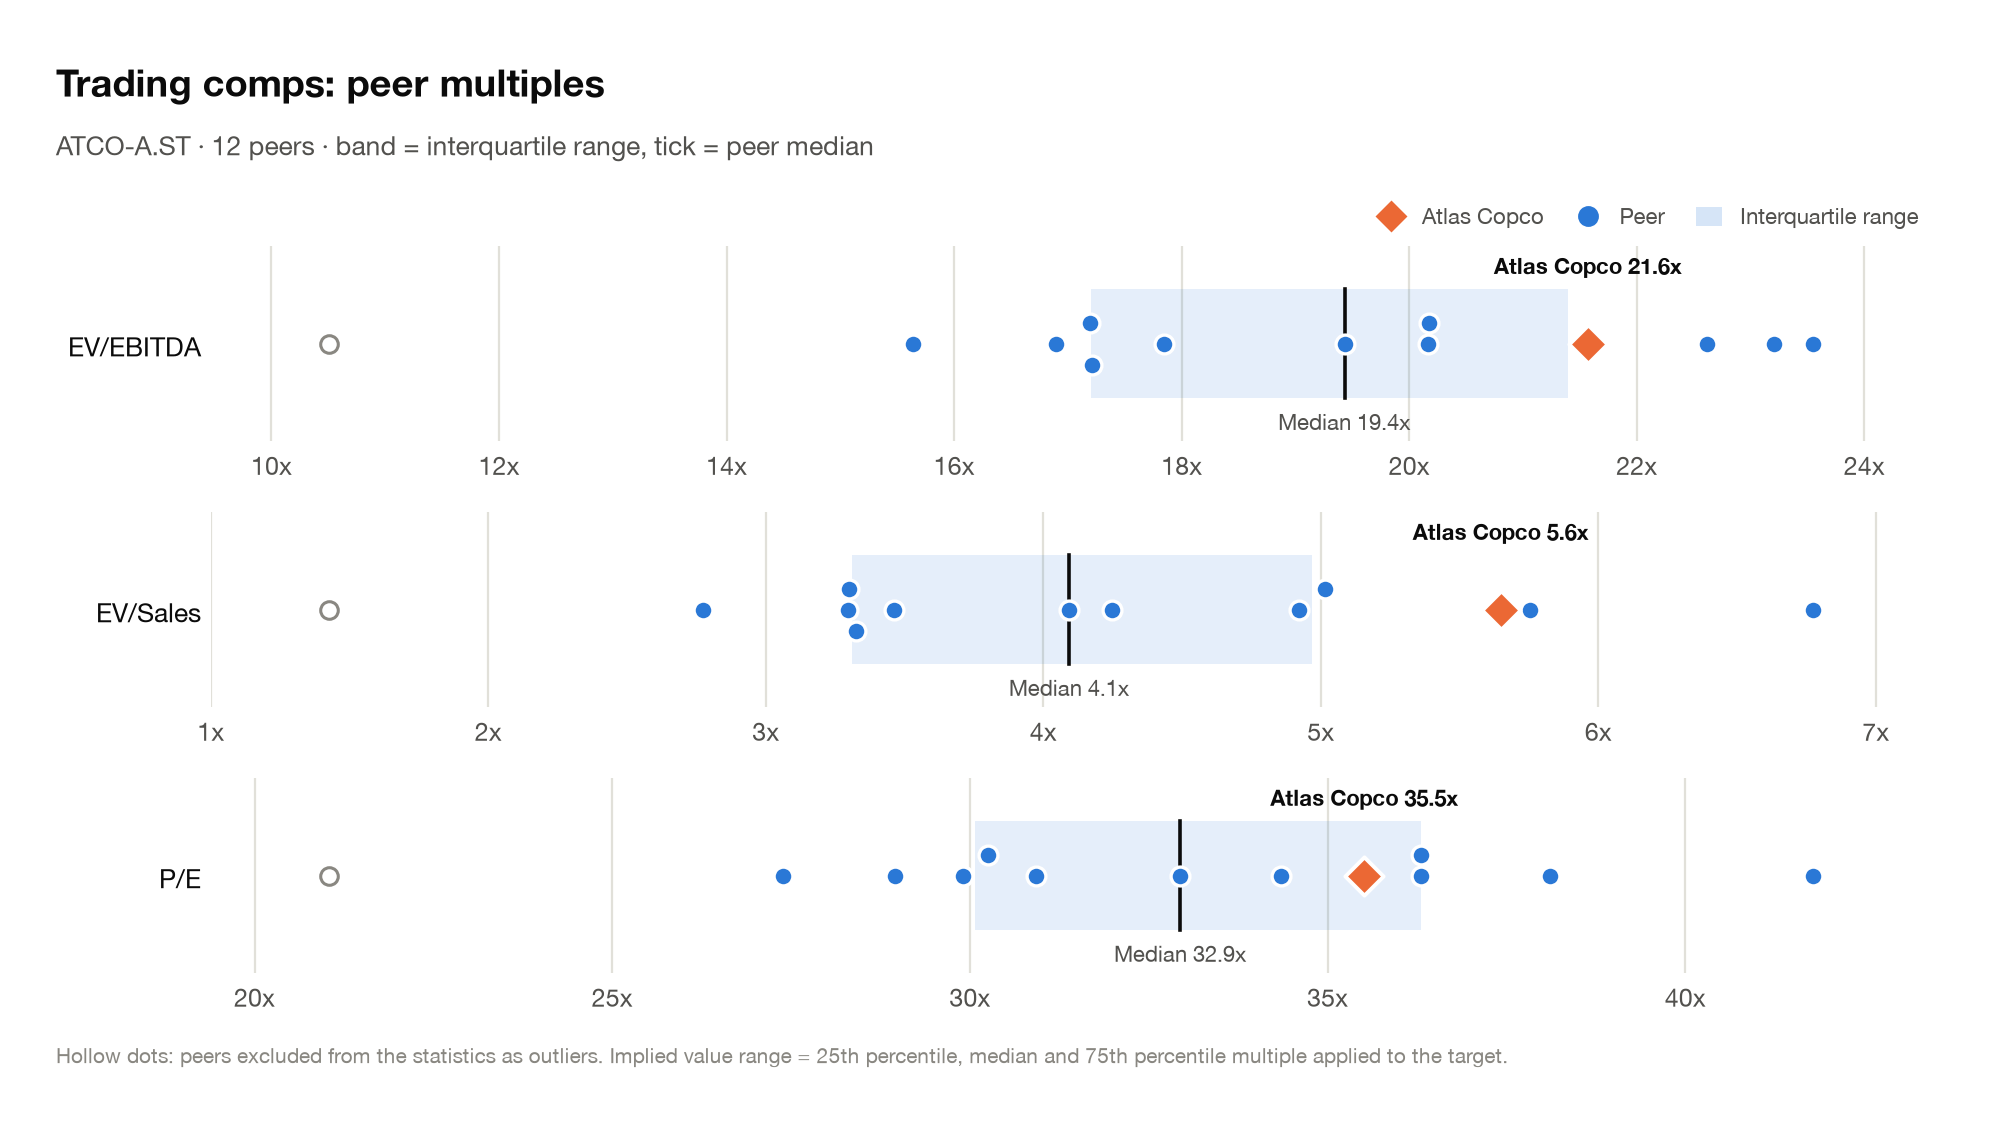
\includegraphics[width=\linewidth]{comps_peer_multiples.png}
\caption{Jämförelsebolagens multiplar. Bandet är kvartilavståndet, strecket medianen och
romben Atlas Copco, som ligger ungefär vid gruppens 75:e percentil på EV/EBITDA och P/E. Den
ofyllda punkten är bolaget som rensades bort.}
\label{fig:comps}
\end{figure}

För banker, försäkringsbolag, investmentbolag och fastighetsbolag räknar motorn bara P/E,
eftersom rörelsevärde och EBITDA inte är meningsfulla när skulden är själva råvaran.
Kandidaterna hämtas då i första hand ur samma branschfamilj (till exempel alla banker), och
klustringen använder bara storlek, avkastning på eget kapital och beta.
